\newpage
\chapter{Разширени графични възможности и вероятностни разпределения}
\label{chapter08}

\section{Разширени графични възможности}

Към базовите графични възможности на R, пакетите ggplot2 и lattice добавят множество допълнителни възможности. Синтаксисът на извикванията леко се различава от този на функциите в базовите възможности, но това създава затруднения само в началния етап от употребата на двата пакета. 

За визуализация, чрез ggplot2 като основа се използва функцията ggplot. В общия случай тази функция получава, като входен параметър данните за визуализиране и понякога някои допълнителни параметри. Резултатът от изпълнението на ggplot е обект, който в последствие може да бъде допълнително променян, чрез добавяне на възможности с помощта на операцията събиране (+). 

\subsection{Хистограми и плътности}

Хистограмата служи за групиране на стойностите и изброяване на това колко стойности попадат по определените групи. Размерът на всяка група (bin) определя ширината на стълба. 

\begin{lstlisting}[caption=Хистограма и плътност, label=listing0150]
library(ggplot2)

ggplot(data=diamonds) + geom_histogram(aes(x=carat))

ggplot(data=diamonds) + geom_density(aes(x=carat),fill="grey50")
\end{lstlisting}

Както и в предходния пример за хистограма, тук също е представено разпределението на диамантите по карати (Листинг \ref{listing0150}).

\begin{figure}[h!]
  \centering
  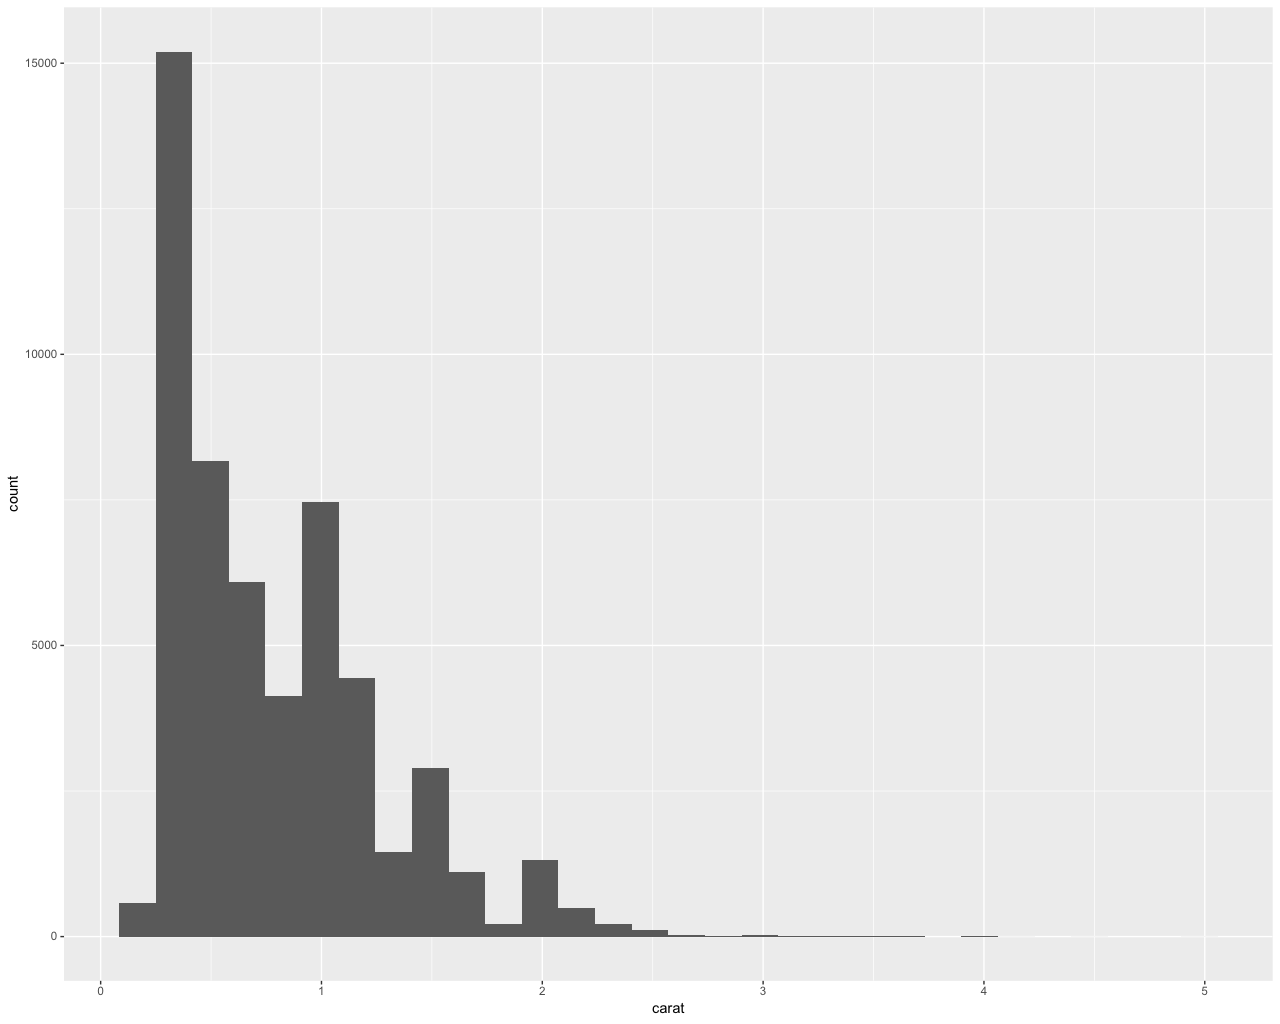
\includegraphics[width=1.0\linewidth]{pic0030}
  \caption{Хистограма при 30 групи}
\label{figure0030}
\end{figure}
\FloatBarrier

Функцията aes определя кои данни да бъдат използвани за разполагане по осите. В примера с диамантите, това е характеристиката за тегло (карат). 

\begin{figure}[h!]
  \centering
  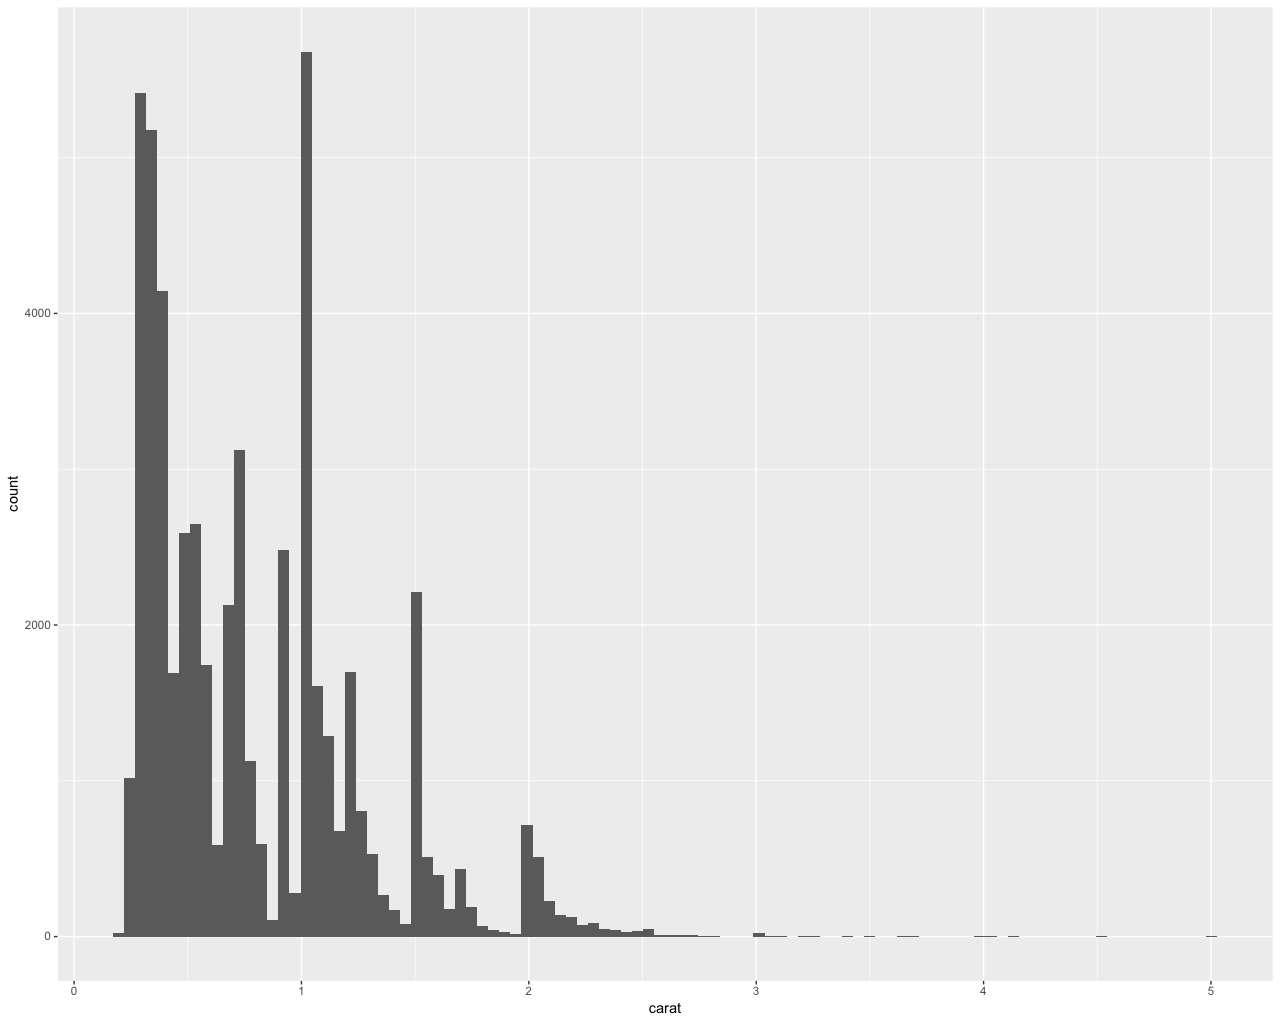
\includegraphics[width=1.0\linewidth]{pic0031}
  \caption{Хистограма при 100 групи}
\label{figure0031}
\end{figure}
\FloatBarrier

Размерът на групите в хистограмата може да варира (Фиг. \ref{figure0030},\ref{figure0031}). За да се изчертае плътностна функция е достатъчно графичният обект, генериран от ggplot, да бъде декориран с функцията geom\_density (Фиг. \ref{figure0032}), вместо с функцията geom\_histogram. 


\begin{figure}[h!]
  \centering
  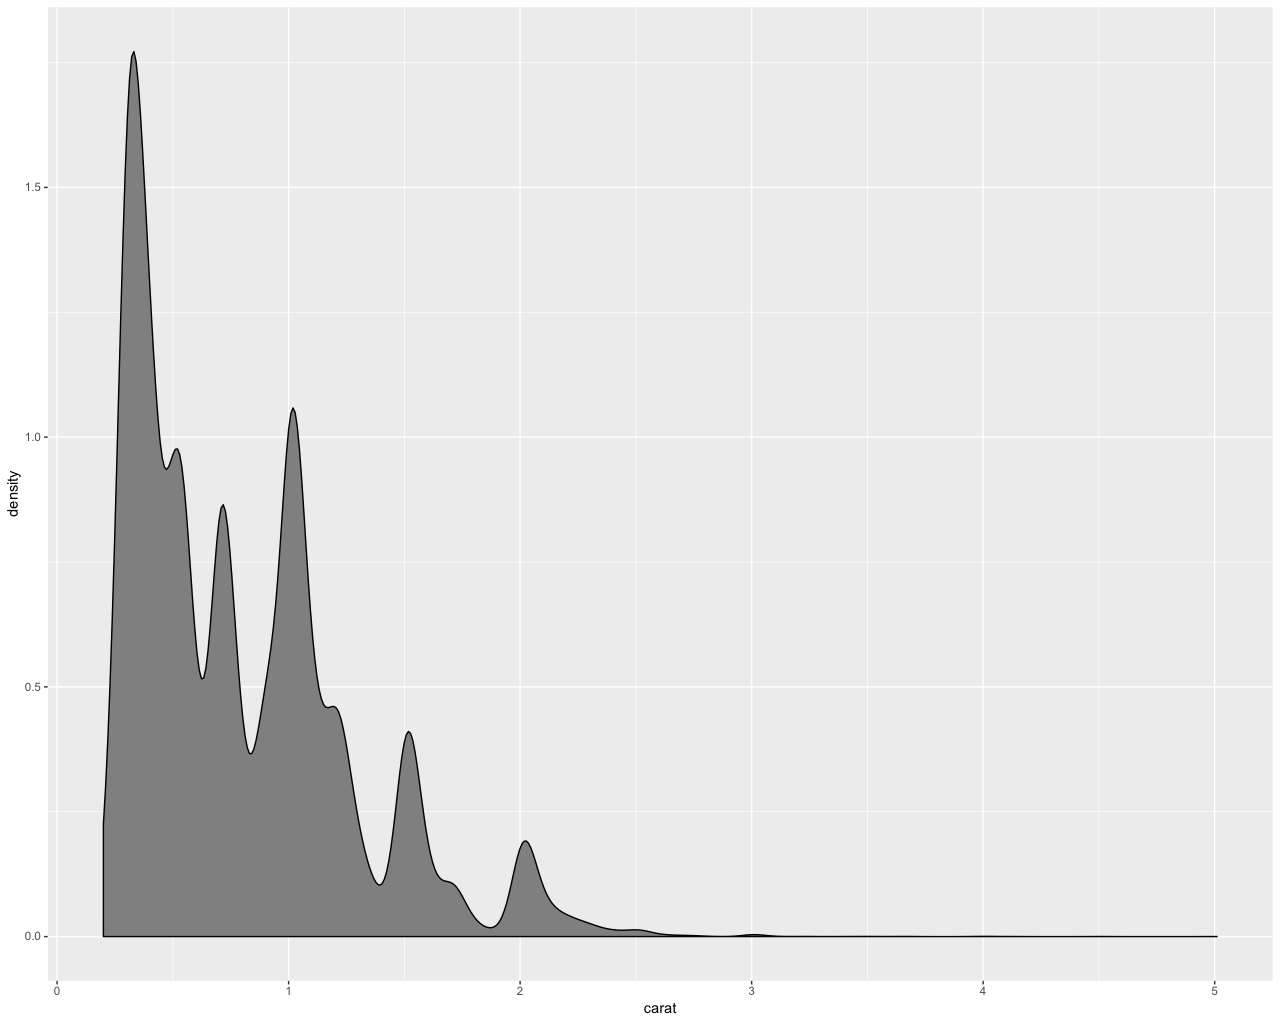
\includegraphics[width=1.0\linewidth]{pic0032}
  \caption{Плътностна функция}
\label{figure0032}
\end{figure}
\FloatBarrier

Хистограмата показва броене по групи, докато плътностната функция задава вероятността определен камък да попадне в предварително определен интервал. Макар и много да си приличат, хистограмата и плътностната функция са подходящи в два различни случая. Хистограмите са полезни при дискретни случайни величини, докато плътностните функции намират повече употреба в непрекъснатите случайни величини. 

\subsection{Диаграми на разсейване}

Пакетът ggplot2 разширява възможностите за визуализация на диаграми на разпръскване, които базовата функционалност на R предлага (Листинг \ref{listing0151}). 

\begin{lstlisting}[caption=Диаграма на разпръскване с ggplot2, label=listing0151]
library(ggplot2)
ggplot(diamonds, aes(x=carat, y=price)) + geom_point()
\end{lstlisting}

Функцията aes определя кои колони от множеството данни да се използват при визуализацията (Фиг. \ref{figure0033}). Пакетът ggplot2 дава и друго много съществено предимство, графиката която ще се изчертава да бъде съхранена в отделен обект, на който обект след това да се добавят различни визуални декорации (обектът c2p от примера).

\begin{figure}[h!]
  \centering
  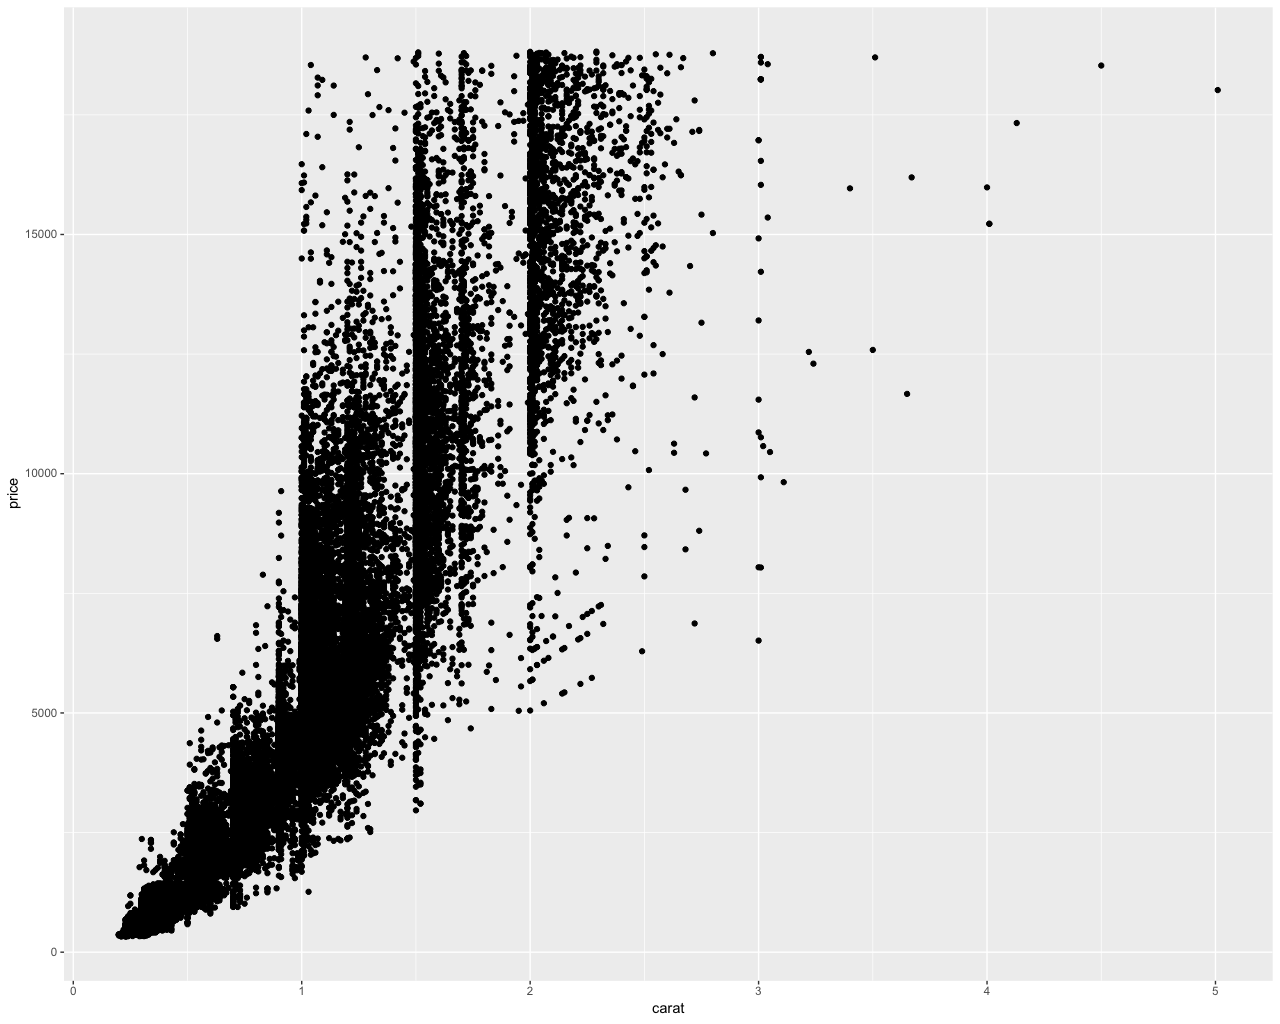
\includegraphics[width=1.0\linewidth]{pic0033}
  \caption{Диаграма на разпръскване с ggplot2}
\label{figure0033}
\end{figure}
\FloatBarrier

Пакетът дава възможности и за подреждането на група от диаграми на разсейването. Това се постига с някоя от функциите facet\_wrap или facetю\_grid (Листинг \ref{listing0152}). 

\begin{lstlisting}[caption=Диаграма на разпръскване групирани по признак, label=listing0152]
c2p <- ggplot(diamonds, aes(x=carat, y=price))

c2p + geom_point(aes(color=color)) + facet_wrap(~color)

c2p + geom_point(aes(color=color)) + facet_grid(clarity~cut)
\end{lstlisting}

Функцията facet\_wrap разделя множеството от данните на групи, според зададения признак (в примера това е цветът на диамантите) и след това формира диаграма на разпръскване за всяка от групите (Фиг. \ref{figure0034}).

\begin{figure}[h!]
  \centering
  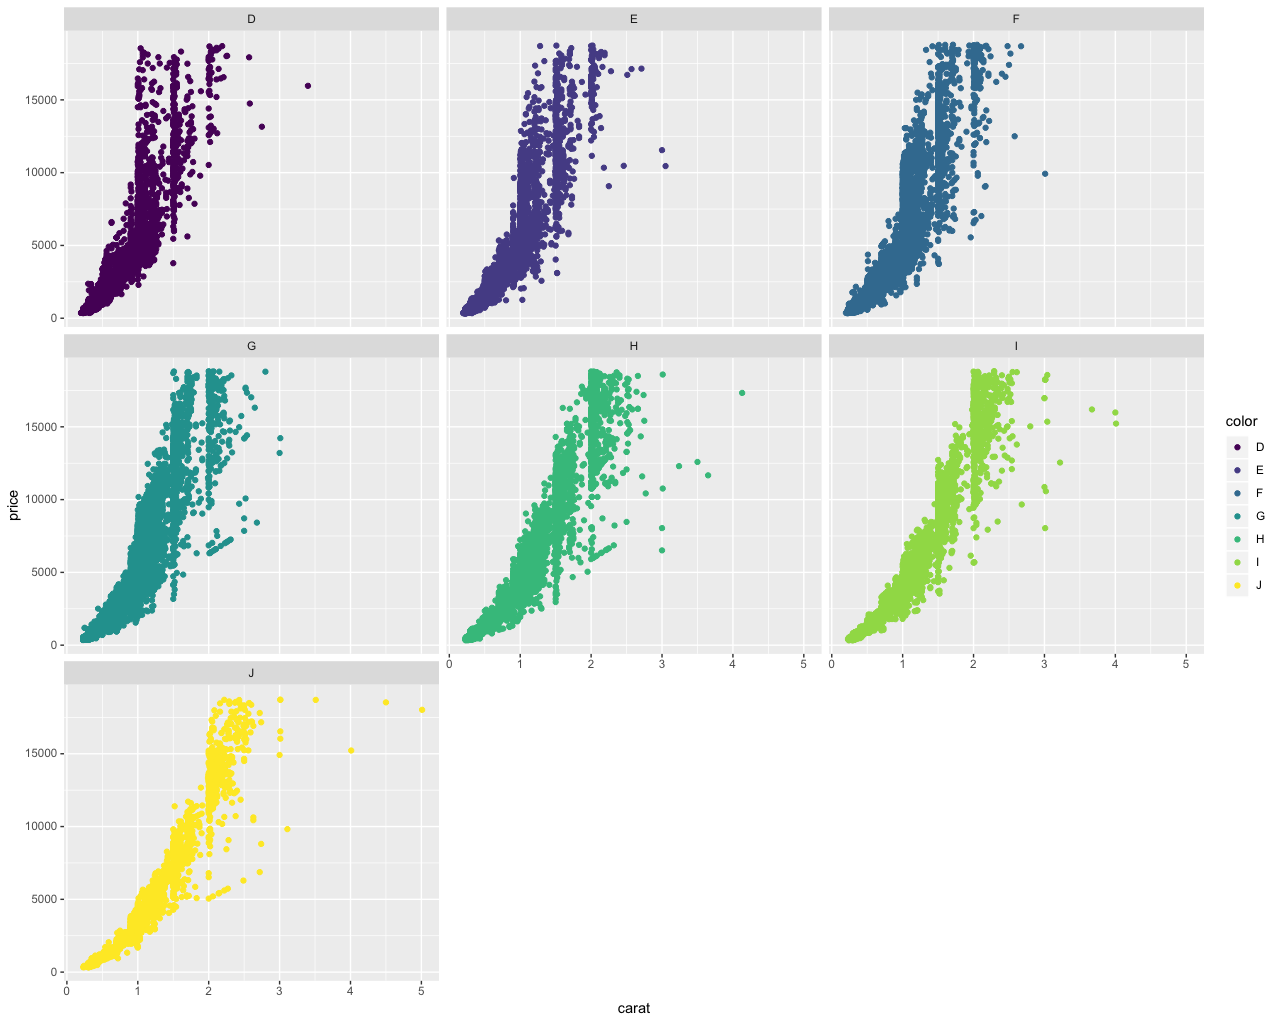
\includegraphics[width=1.0\linewidth]{pic0034}
  \caption{Диаграма на разпръскване по групи за цвят на диамантите}
\label{figure0034}
\end{figure}
\FloatBarrier

Функцията facet\_grid действа по сходен начин, но всички стойности на признака за групиране се отразяват на осите за всяка от графиките (Фиг. \ref{figure0035}). Важно е да се забележи начина по който са ориентирани осите на всяка от подграфиките. Ориентацията пряко зависи дали признакът за чистота е от ляво, а признакът за качество на среда от дясно или обратното. 

\begin{figure}[h!]
  \centering
  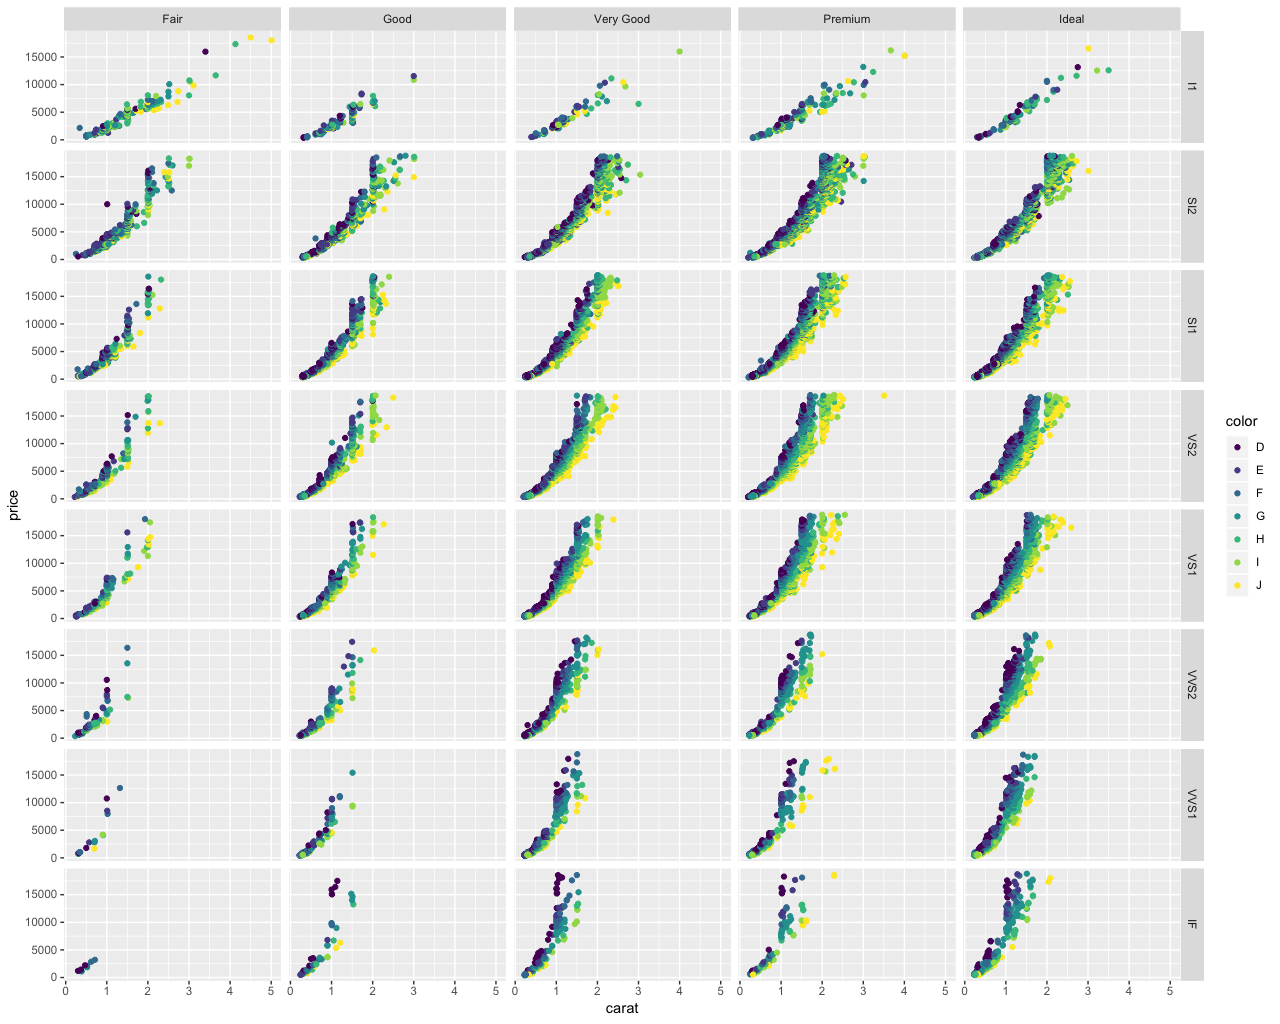
\includegraphics[width=1.0\linewidth]{pic0035}
  \caption{Визуализация с групиране по два признака}
\label{figure0035}
\end{figure}
\FloatBarrier

Организацията на графики по групи е възможна с различни графични представяния, като пример е представянето на хистограма в групи по качество на сряза (Фиг. \ref{figure0036}).

\begin{figure}[h!]
  \centering
  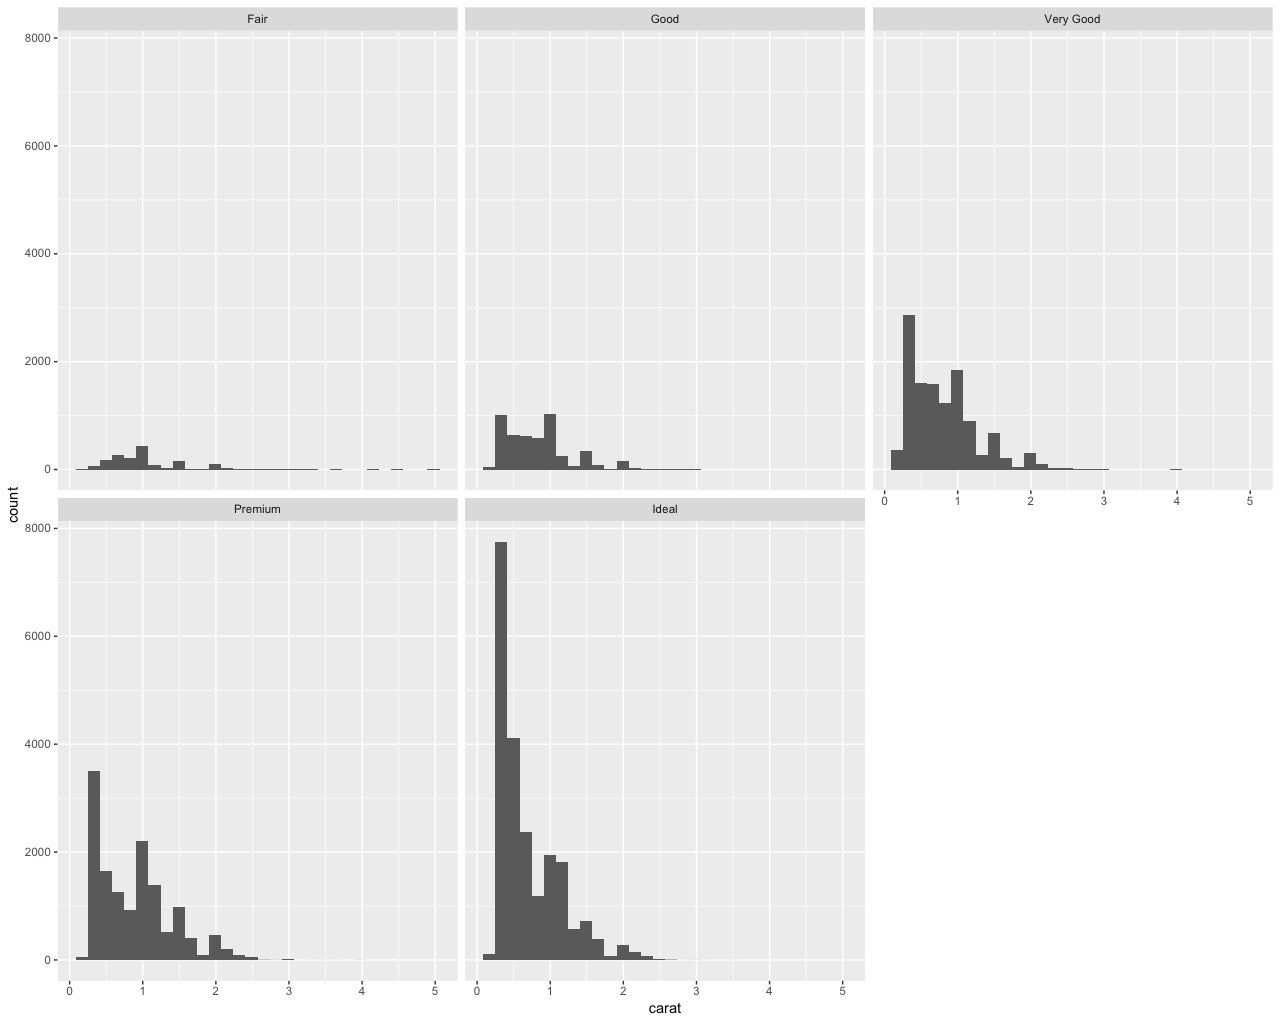
\includegraphics[width=1.0\linewidth]{pic0036}
  \caption{Визуализация на хистограми с групиране}
\label{figure0036}
\end{figure}
\FloatBarrier

\subsection{Графики тип кутия и цигулка}

Пакетът ggplot2 дава възможност за визуализация на графики тип кутия (Листинг \ref{listing0153}).

\begin{lstlisting}[caption=Визуализация тип кутия, label=listing0153]
ggplot(diamonds, aes(y=depth)) + geom_boxplot()

ggplot(diamonds, aes(y=depth, x=cut)) + geom_boxplot()

ggplot(diamonds, aes(y=depth, x=cut)) + geom_boxplot() + geom_violin()

ggplot(diamonds, aes(y=depth, x=cut))+ geom_point() + geom_violin()
\end{lstlisting}

При обща визуализация на данните, без да се търси групиране по признан за абсцисната ос може да не се подава стойност (Фиг. \ref{figure0037}). 

\begin{figure}[h!]
  \centering
  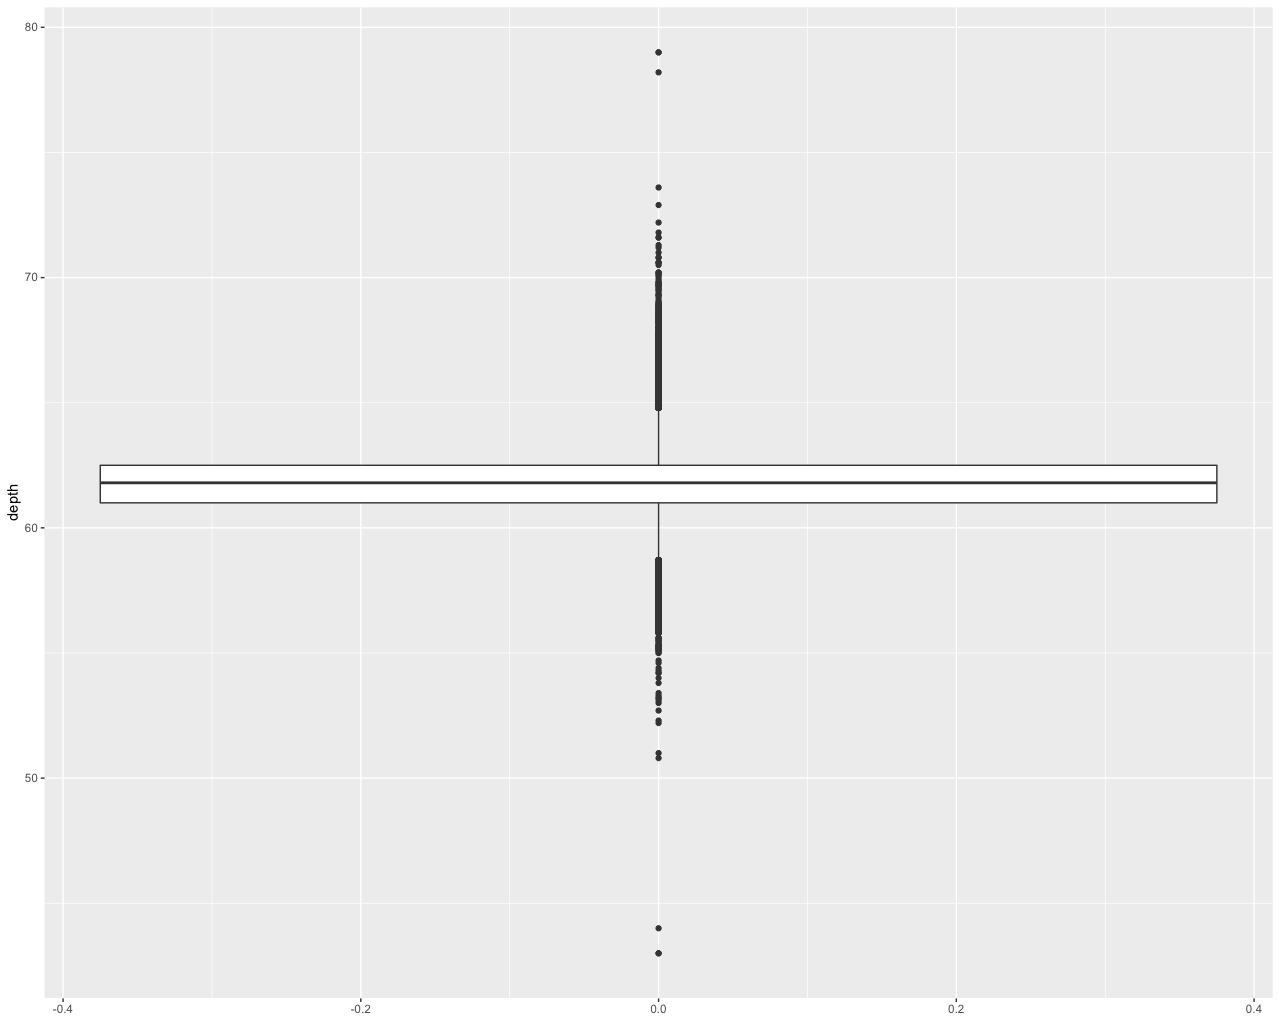
\includegraphics[width=1.0\linewidth]{pic0037}
  \caption{Визуализация на характеристиката за дълбочина на диамантите}
\label{figure0037}
\end{figure}
\FloatBarrier

Визуализацията на графики от тип кутия, с групиране по признак се реализира чрез подаване на колоната, по която да се групира, като параметър за абцисна ос, на функцията aes (Фиг. \ref{figure0038}).

\begin{figure}[h!]
  \centering
  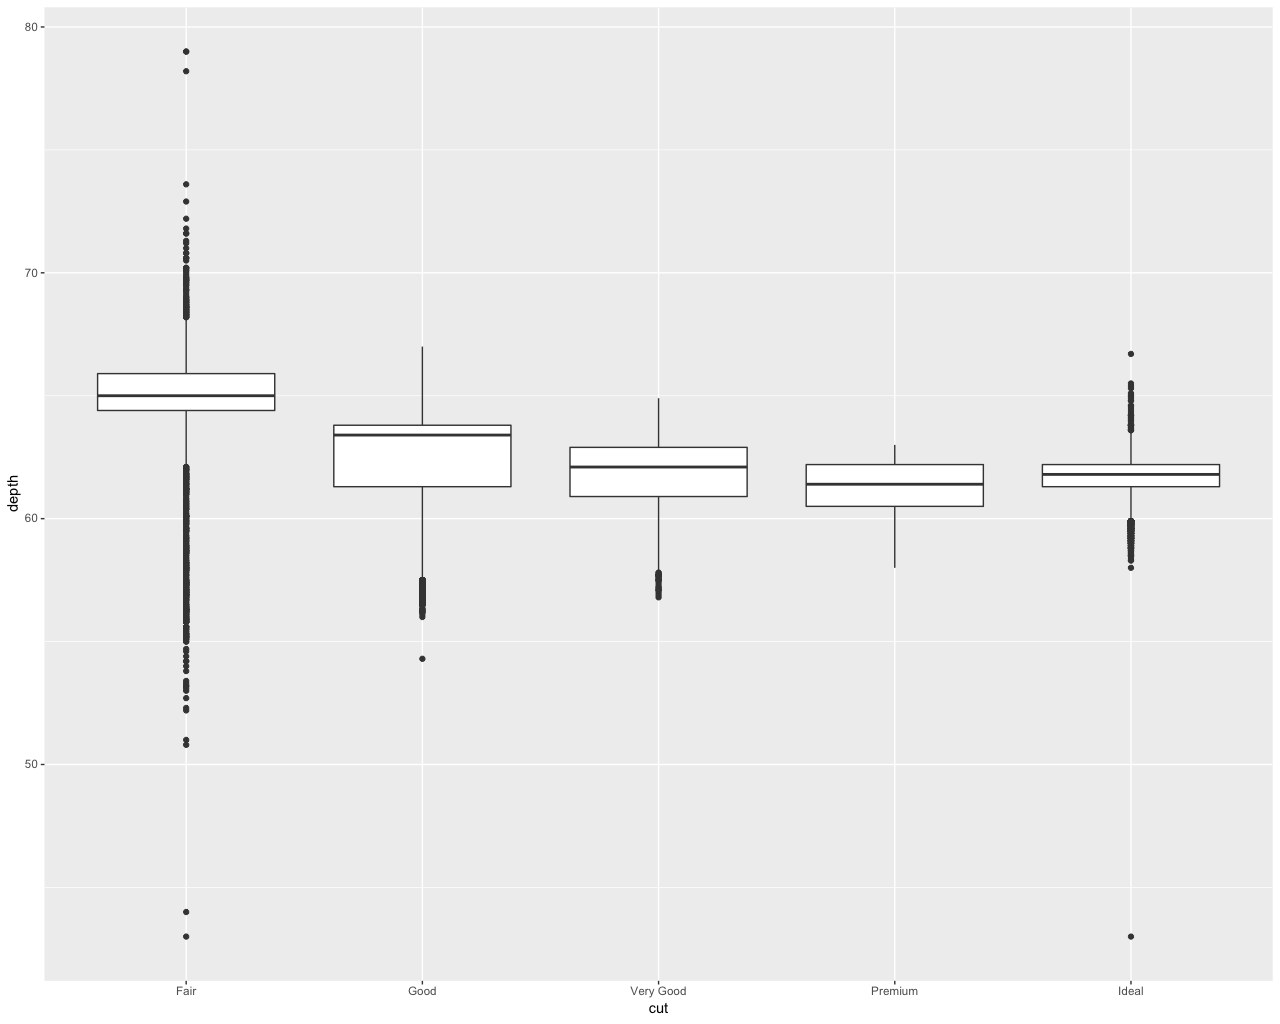
\includegraphics[width=1.0\linewidth]{pic0038}
  \caption{Dълбочина на диамантите в групи според сряза}
\label{figure0038}
\end{figure}
\FloatBarrier

От графика тип кутии много лесно се преминава към графика от тип цигулки, чрез подмяна на декориращата функция (Фиг. \ref{figure0039}).

\begin{figure}[h!]
  \centering
  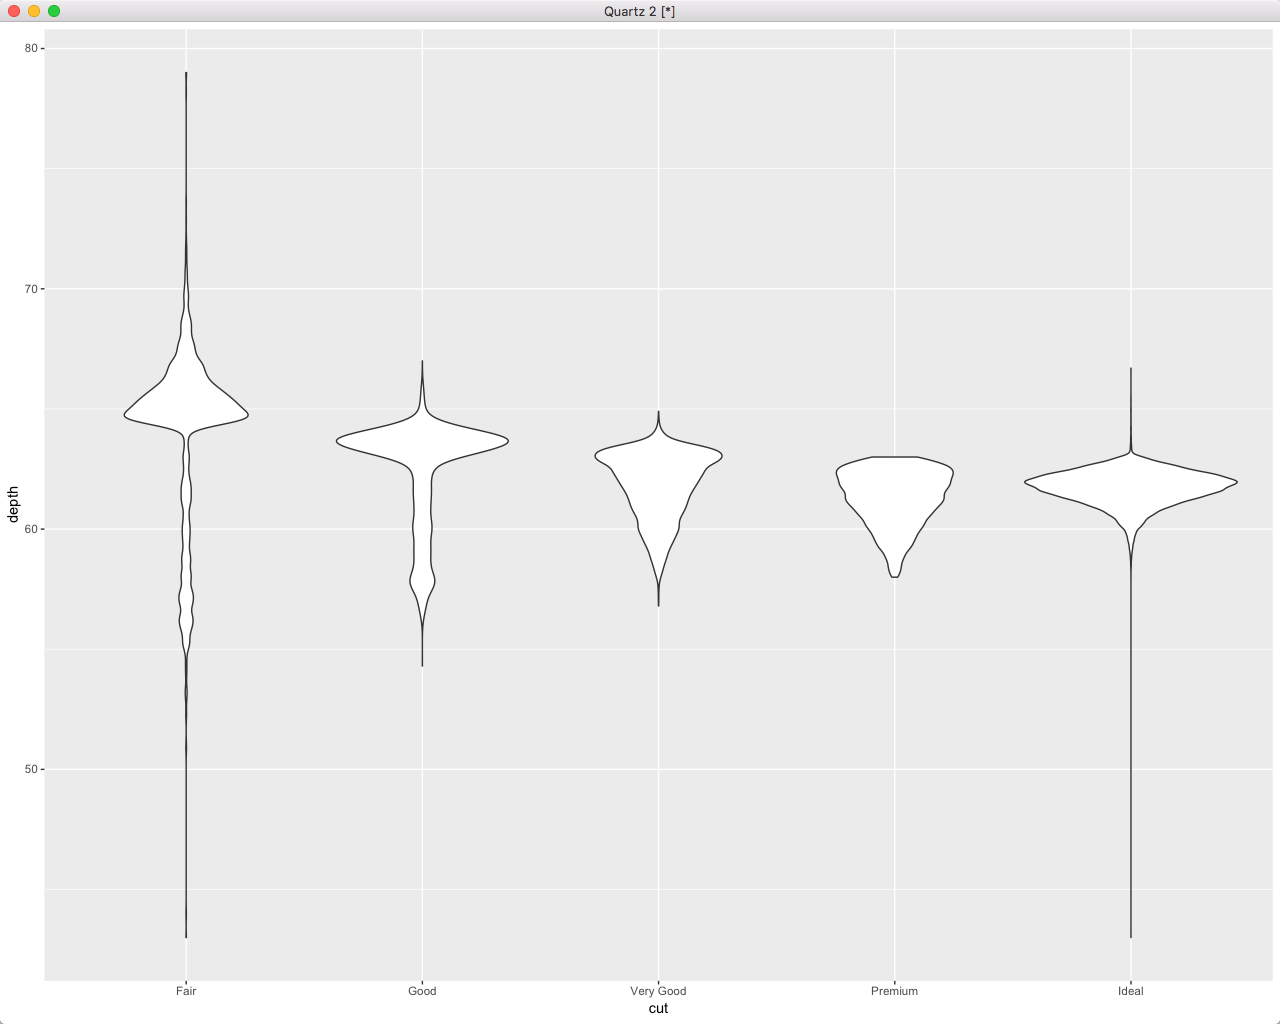
\includegraphics[width=1.0\linewidth]{pic0039}
  \caption{Графика тип цигулки}
\label{figure0039}
\end{figure}
\FloatBarrier

Графиките тип кутия и тип цигулка си приличат, като основната разлика е, че цигулките имат повече смисъла на плътностна функция и носят повече информация, отколкото правите ръбове на кутиите. 

\begin{figure}[h!]
  \centering
  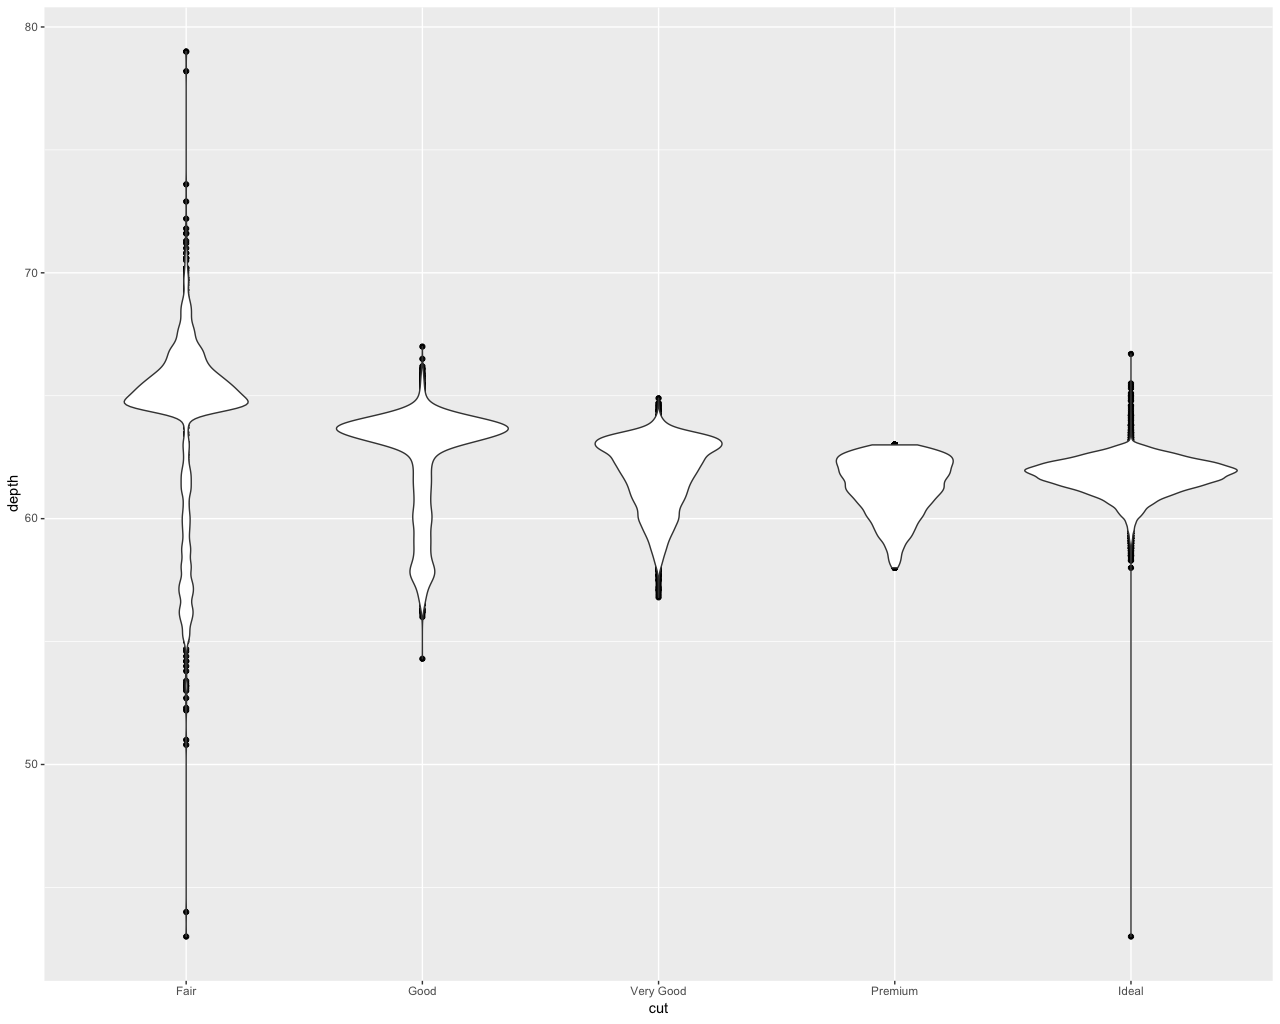
\includegraphics[width=1.0\linewidth]{pic0040}
  \caption{Добавяне на декорация с точки}
\label{figure0040}
\end{figure}
\FloatBarrier

Декорациите за визуализация на данните може да се наслагват една върху друга, като от съществено значение е редът на изчертаването им (Фиг. \ref{figure0040}). Ако декорацията с точките бъде добавена след декорацията с цигулките, точки ще се появят и върху самите цигулки. 

\section*{Заключение}

